\documentclass[a4paper, 12pt]{article}

\usepackage[table,xcdraw]{xcolor}
\usepackage{enumerate}
\usepackage{graphicx}
\usepackage[T5]{fontenc}
\usepackage[utf8]{inputenc}
\usepackage[margin = 2cm]{geometry}
\usepackage{amsfonts, amsmath, amssymb}
\usepackage[none]{hyphenat}
\usepackage{fancyhdr}
\usepackage{float}
\usepackage{hyperref}
\usepackage{caption}
\usepackage[nottoc, notlot, notlof]{tocbibind}

\captionsetup[table]{skip=5pt}
\pagestyle{fancy}
\fancyhead[L]{Trường Đại học Khoa học Tự nhiên - ĐHQG TP.HCM}
\fancyhead[R]{Nhóm Just $4^{th}$}

\begin{document}
\begin{titlepage}
	\begin{center}
		\vspace*{1cm}
		\Large\textbf{Báo cáo \#2\\Thiết kế hệ thống}\\
		
		\vfill
		\line(1,0){450}\\[4mm]
		\LARGE\textbf{\MakeUppercase{Dự án quản lý tạp chiếu phim}}\\[3mm]
		\Large{Nhập môn Công nghệ phần mềm (CSC13002)}\\[3mm]
		\Large{Nhóm Just $4^{th}$}
		\line(1,0){430}\\
		\vfill
		
		\vfill
		TP Hồ Chí Minh, ngày 07/11/2020
	\end{center}
\end{titlepage}

\tableofcontents
\thispagestyle{empty}
\clearpage

\section{Thông tin nhóm}
\label{sec:info}
\begin{enumerate}
	\item \textbf{Đường link GitHub}: \url{https://github.com/baolongnguyenmac/CinemaManagementSystem}
	\item \textbf{Đường link Trello}: \url{https://trello.com/b/uymvzWAR/báo-cáo-thiết-kế-hệ-thống}
	\item \textbf{Danh sách thành viên}
	\begin{table}[H]
		\begin{center}
			\begin{tabular}{|c|c|l|c|c|}
				\hline
				STT & MSSV     & \multicolumn{1}{c|}{Họ tên} & Email                         & SĐT        \\ \hline
				1   & 18120201 & Nguyễn Bảo Long             & 18120201@student.hcmus.edu.vn & 0919070940 \\ \hline
				2   & 18120211 & Võ Thế Minh                 & 18120211@student.hcmus.edu.vn & 0981850699 \\ \hline
				3   & 18120227 & Phạm Văn Minh Phương        & 18120227@student.hcmus.edu.vn & 0343049359 \\ \hline
				4   & 18120210 & Phạm Tống Bình Minh         & 18120210@student.hcmus.edu.vn & 0971877781 \\ \hline
				5   & 18120264 & Nguyễn Duy Vũ               & 18120264@student.hcmus.edu.vn & 0911572108 \\ \hline
			\end{tabular}
			\caption{Bảng danh sách thành viên nhóm}
		\end{center}
	\end{table}
\end{enumerate}
\clearpage

\section{Lịch sử cập nhật}
\label{sec:history}
\begin{table}[h]
	\begin{center}
		\begin{tabular}{|c|c|c|l|l|}
			\hline
			STT &Ngày cập nhật &Phiên bản &\multicolumn{1}{c|}{Mô tả chi tiết} &\multicolumn{1}{c|}{Tác giả} \\ \hline
			1 &11/11/2020 &1.0 &\begin{tabular}[c]{@{}l@{}}- Kiến trúc hệ thống\\ - Nhận diện hệ thống con\\ - Ánh xạ với phần cứng\\ - Thiết kế database\end{tabular} &\begin{tabular}[c]{@{}l@{}}Phạm Tống Bình Minh\\ Nguyễn Duy Vũ\end{tabular} \\ \hline
			2 &14/11/2020 &1.1 &\begin{tabular}[c]{@{}l@{}}- Xác định giao thức mạng\\ - Vẽ biểu đồ use case\\- Vẽ biểu đồ tuần tự\\ - Lên kế hoạch làm việc\end{tabular} &\begin{tabular}[c]{@{}l@{}}Phạm Tống Bình Minh\\ Nguyễn Duy Vũ\\Nguyễn Bảo Long \\ Võ Thế Minh\end{tabular} \\ \hline
			% 3 &25/10/2020 &1.2 &\begin{tabular}[c]{@{}l@{}}- Đặc tả giao diện người dùng\\ - Lên kế hoạch làm việc\end{tabular} &\begin{tabular}[c]{@{}l@{}}Nguyễn Bảo Long \\ Võ Thế Minh \\ Phạm Văn Minh Phương\end{tabular} \\ \hline
			% 4 &30/10/2020 &1.3 &- Đặc tả giao diện người dùng &Phạm Văn Minh Phương \\ \hline
			% 5 &31/10/2020 &1.5 &- Phân tích đóng góp cá nhân &Phạm Văn Minh Phương \\ \hline
		\end{tabular}
		\caption{Bảng lịch sử cập nhật các phiên bản của báo cáo yêu cầu}
	\end{center}
\end{table}
\clearpage

\section{Phân tích đóng góp cá nhân}
\label{sec:analys}
\begin{table}[H]
	\begin{center}
		\begin{tabular}{|c|l|l|c|}
			\hline
			STT & \multicolumn{1}{c|}{Họ tên} & \multicolumn{1}{c|}{Công việc tham gia}                                                & Phần trăm đóng góp \\ \hline
			% 1 & Nguyễn Bảo Long      & \begin{tabular}[c]{@{}l@{}}- Mô tả bài toán\\ - Mô tả yêu cầu hệ thống\\ - Vẽ biểu đồ tuần tự\end{tabular}              & 20\% \\ \hline
			% 2 & Phạm Văn Minh Phương & \begin{tabular}[c]{@{}l@{}}- Nhận diện thành viên\\ - Đặc tả giao diện người dùng\end{tabular}                          & 20\% \\ \hline
			% 3   & Võ Thế Minh                 & \begin{tabular}[c]{@{}l@{}}- Vẽ biểu đồ tuần tự\\ - Lên kế hoạch làm việc\end{tabular} & 20\%               \\ \hline
			% 4 & Phạm Tống Bình Minh  & \begin{tabular}[c]{@{}l@{}}- Đặc tả use case\\ - Vẽ ma trận truy vết\\ - Vẽ biểu đồ use case\end{tabular}               & 20\% \\ \hline
			% 5 & Nguyễn Duy Vũ        & \begin{tabular}[c]{@{}l@{}}- Lên danh sách actor, stakeholder\\ - Đặc tả use case \\ - Vẽ ma trận truy vết\end{tabular} & 20\% \\ \hline
		\end{tabular}
		\caption{Bảng phân tích đóng góp cá nhân}
	\end{center}
\end{table}
\clearpage

\section{Thiết kế kiến trúc và hệ thống}

\subsection{Kiến trúc hệ thống}
\begin{figure}[H]
	\begin{center}
		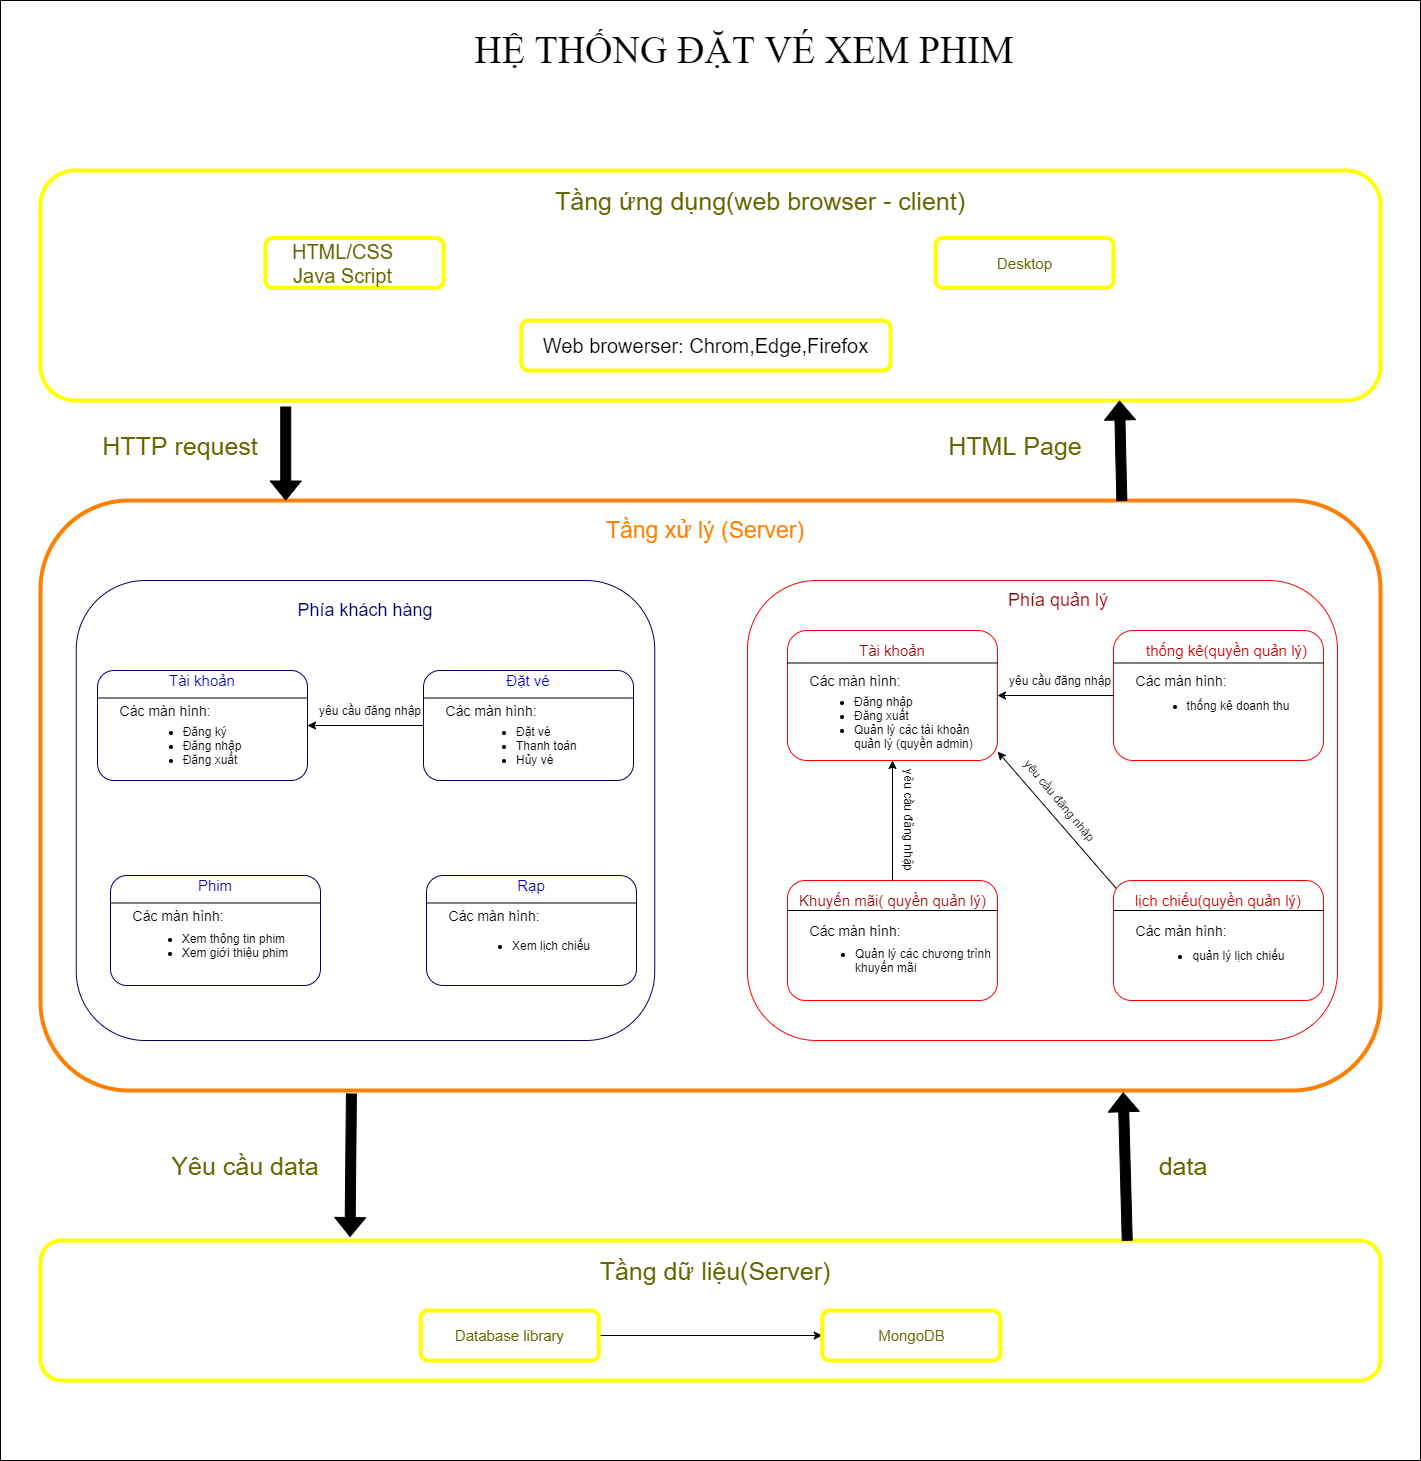
\includegraphics[scale = 0.25]{image/4.1.png}
		\caption{Kiến trúc tổng thể hệ thống}
	\end{center}
\end{figure}

Hệ thống đặt vé xem phim sử dụng kiến trúc Client - Server:
\begin{itemize}
	\item Ở phía Client sử dụng Web Browser được mở từ các thiết bị (PC, Laptop, SmartPhone,...) để truy cập vào trang web.
	\item Ở phía Server sẽ xử lý các yêu cầu (HTTP request) được gửi từ Client thông qua các module và trả về các page HTML hiện thị trên Web Browser.Ở hệ thống này nhóm dùng node.js để xây dựng hệ thống.
	\item Quá trình xử lý ở Server có thể yêu cầu truy xuất cơ sở dữ liệu (CRUD) được lưu ở hệ quản trị cơ sở dữ liệu. Ở hệ thống này nhóm dùng hệ quản trị cơ sở dữ liệu MySQL.
\end{itemize}

\subsection{Nhận diện hệ thống con}
\begin{figure}[H]
	\begin{center}
		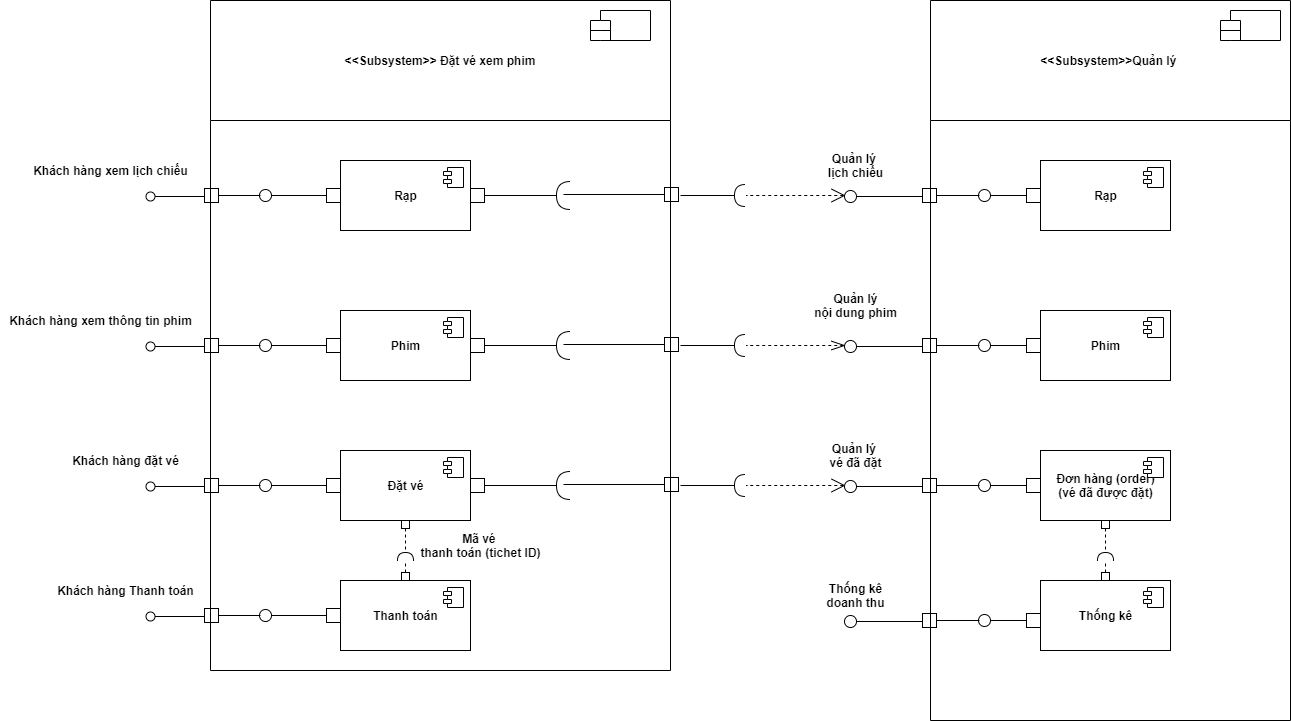
\includegraphics[scale = 0.35]{image/4.2.png}
		\caption{Component Diagram}
	\end{center}
\end{figure}

Hệ thống đặt vé xem phim có 2 hệ thống con :
\begin{itemize}
	\item Hệ thống con đặt vé xem phim với các component:
	\begin{enumerate}
		\item Rạp : cung cấp chức năng xem lịch chiếu. 
		\item Phim : cung cấp chức năng xem thông tin phim.
		\item Đặt vé : cung cấp chức năng đặt vé.
		\item Thanh Toán : cung cấp chức năng thanh toán.
	\end{enumerate}
	\item Hệ thống con quản lý với các component
	\begin{enumerate}
		\item Rạp : cung cấp chức năng xem lịch chiếu.
		\item Phim: cung cấp chức năng xem lịch chiếu.
		\item Đơn hàng:cung cấp chức năng xem quản lý vé đã đặt.
		\item Thống kê: cung cấp chức năng thống kê doanh thu.
	\end{enumerate}
\end{itemize}

\subsection{Ánh xạ các phần của hệ thống với phần cứng}
\begin{figure}[H]
	\begin{center}
		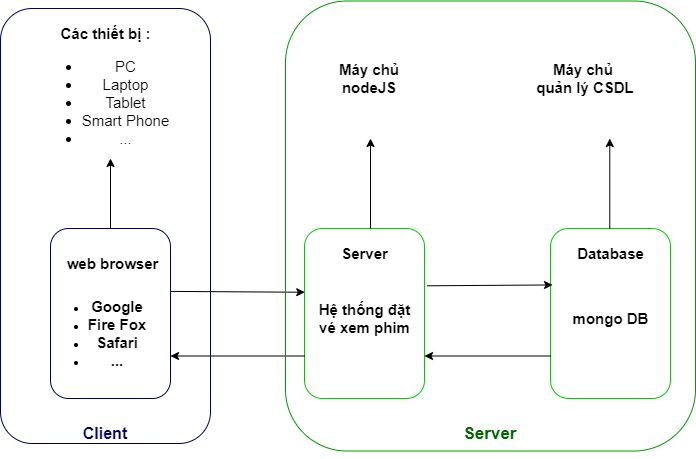
\includegraphics[scale = 0.5]{image/4.3.png}
		\caption{Ánh xạ hệ thống tới phần cứng}
	\end{center}
\end{figure}

Hệ thống đặt vé xem phim sử dụng mô hình Client - Server thì có các phần cứng :
\begin{itemize}
	\item Ở phía Client sẽ sử dụng các thiết bị như Laptop, PC, SmartPhone , Table, ... để truy cập vào hệ thống thông qua Web Browser như Google, Safari, FireFox ...
	\item Ở phía Server sẽ sử dụng các máy chủ để chạy Server và hệ quản trị cơ sở dữ liệu.
\end{itemize}

\subsection{Lưu trữ dữ liệu lâu dài}
\begin{figure}[H]
	\begin{center}
		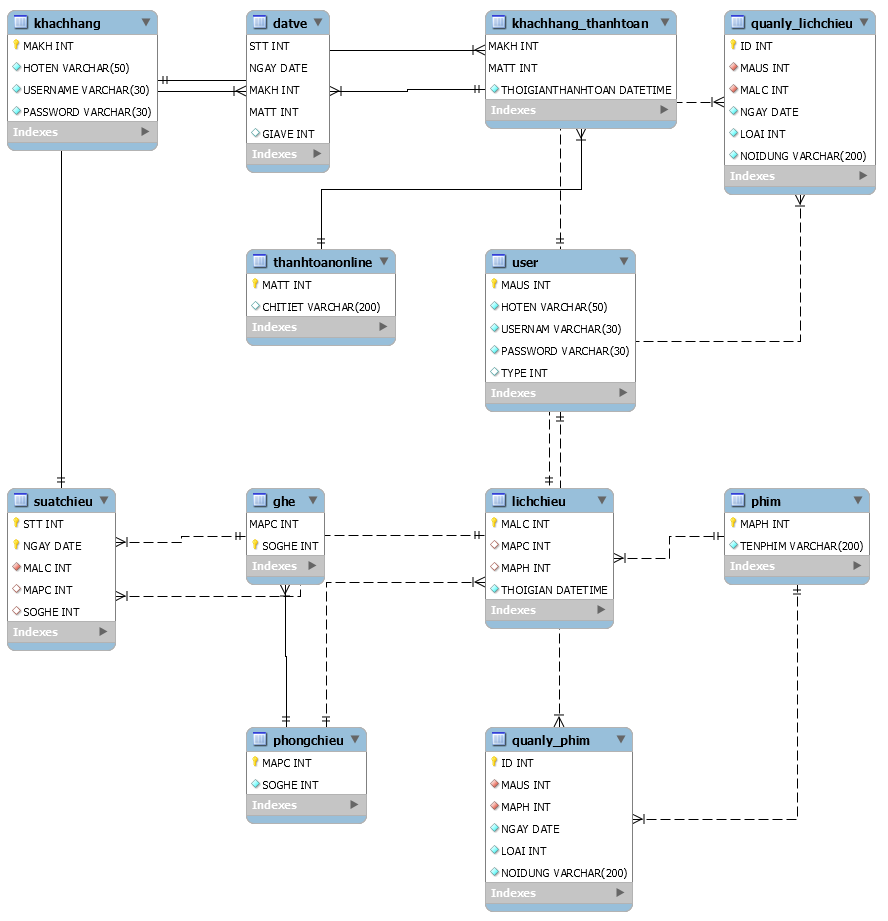
\includegraphics[scale = 0.25]{image/4.4.png}
		\caption{Database Diagram}
	\end{center}
\end{figure}

Hệ thống đặt vé xem phim sử dụng MySQL làm hệ quản trị CSDL với các Table:
\begin{itemize}
	\item PHIM: lưu thông tin Phim.
	\item PHONGCHIEU: lưu thông tin phòng chiếu.
	\item GHE: lưu thông tin về ghế trong PHONGCHIEU.
	\item LICHCHIEU: lưu thông tin lịch chiếu.
	\item SUATCHIEU: lưu thông tin suất chiếu.
	\item DATVE: lưu thông tin đặt vé của khách hàng.
	\item KHACHHANG\_THANHTOAN: lưu thông tin về thanh toán của vé đã đặt.
	\item THANHTOANONLINE: lưu thông tin về thanh toán online cho 1 đơn hàng(đặt vé) thông qua KHACHHANG\_THANHTOAN.
	\item KHACHHANG: lưu thông tin về khách hàng
	\item USER: lưu thông tin về Quản lý và Admin
	\item QUANLIPHIM: lưu lịch sử của việc quản lý (thêm, xóa, sửa) phim.
	\item QUANLILICHCHIEU: lưu lịch sử của việc quản lý (thêm, xóa, sửa) lịch chiếu.
\end{itemize}	

\subsection{Giao thức mạng}

Hệ thống sử dụng các giao thức mạng như sau:
\begin{itemize}
	\item Transmission Control Protocol (TCP): Giao thức điều khiển truyền vận. Chúng là giao thức cốt lõi của Internet Protocol Suite (Bộ giao thức liên mạng). Với nhiệm vụ thực thi mạng, bổ sung cho Internet Protocol. Giao thức này đảm bảo chuyển giao dữ liệu tới nơi nhận một cách đáng tin cậy và đúng thứ tự.
	\item Internet Protocol (IP): Giao thức chính trong Internet protocol suite. Với khả năng chuyển tiếp dữ liệu qua mạng và giúp thiết lập internet thông qua việc định tuyến  của Internet Protocol. IP cung cấp một dịch vụ gửi dữ liệu không đảm bảo  nên gói dữ liệu có thể đến nơi mà không còn nguyên vẹn, nó có thể đến không theo thứ tự.
	\item File Transfer Protocol (FTP): Giao thức truyền tập tin để trao đổi tập tin qua mạng lưới truyền thông dùng giao thức TCP/IP.
	\item Hypertext Transfer Protocol (HTTP): Giao thức truyền tải siêu văn bản. Chúng là một trong năm giao thức chuẩn của mạng Internet. Giao thức này dùng để liên hệ thông tin giữa máy cung cấp dịch vụ (Web server) và Máy sử dụng dịch vụ (Web client). Chúng hoạt trông trong mô hình Client/Server dùng cho World Wide Web.
	\item Hypertext Transfer Protocol over SSL/TLS (HTTPS): Một giao thức kết hợp giữa giao thức HTTP và giao thức bảo mật SSL hay TLS cho phép trao đổi thông tin một cách bảo mật trên Internet.
\end{itemize}
\clearpage

\subsection{Luồng điều khiển (Global Control Flow)}

\begin{itemize}
	\item Thứ tự thực thi: Hệ thống hướng sự kiện: Chờ sự kiện xảy ra và xử lý các sự kiện đó
	\item Phụ thuộc thời gian: Không 
	\item Sử dụng đa luồng: Không 
\end{itemize}

\begin{figure}[H]
	\begin{center}
		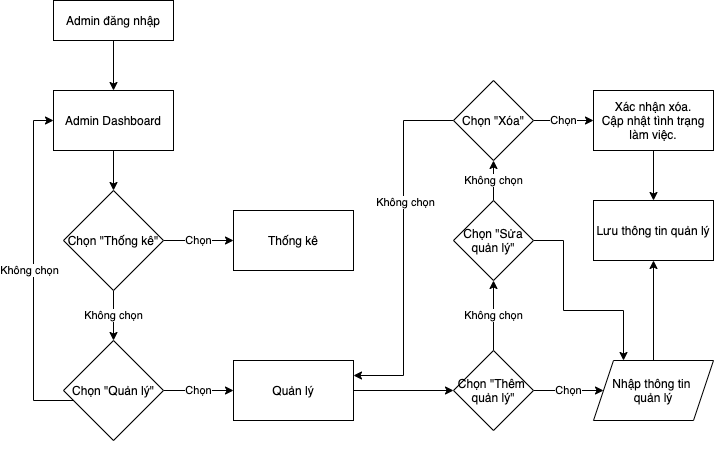
\includegraphics[scale = 0.6]{GCF Charts/GCF_Admin.png}
		\caption{Luồng điều khiển của Admin}
	\end{center}
\end{figure}

\begin{figure}[H]
	\begin{center}
		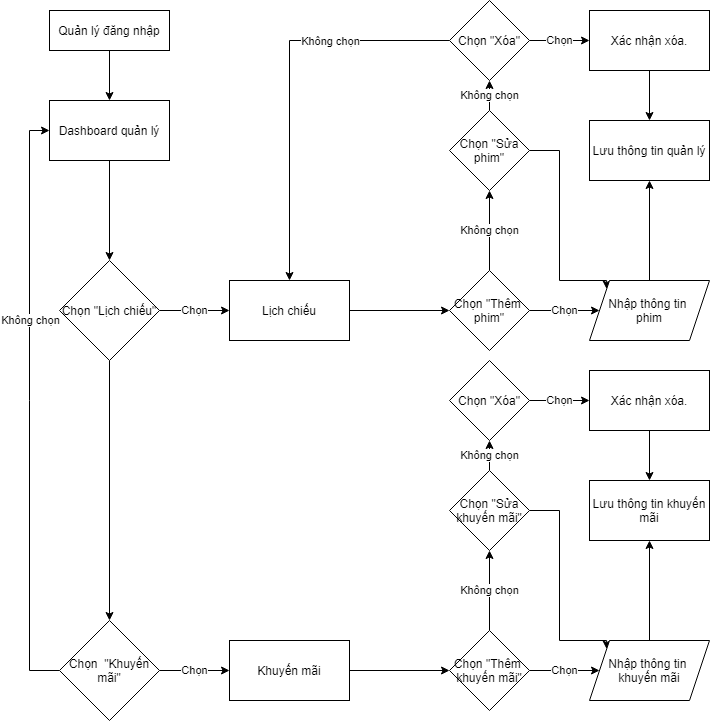
\includegraphics[scale = 0.6]{GCF Charts/GCF_Manager.png}
		\caption{Luồng điều khiển của Quản lý}
	\end{center}
\end{figure}

\begin{figure}[H]
	\begin{center}
		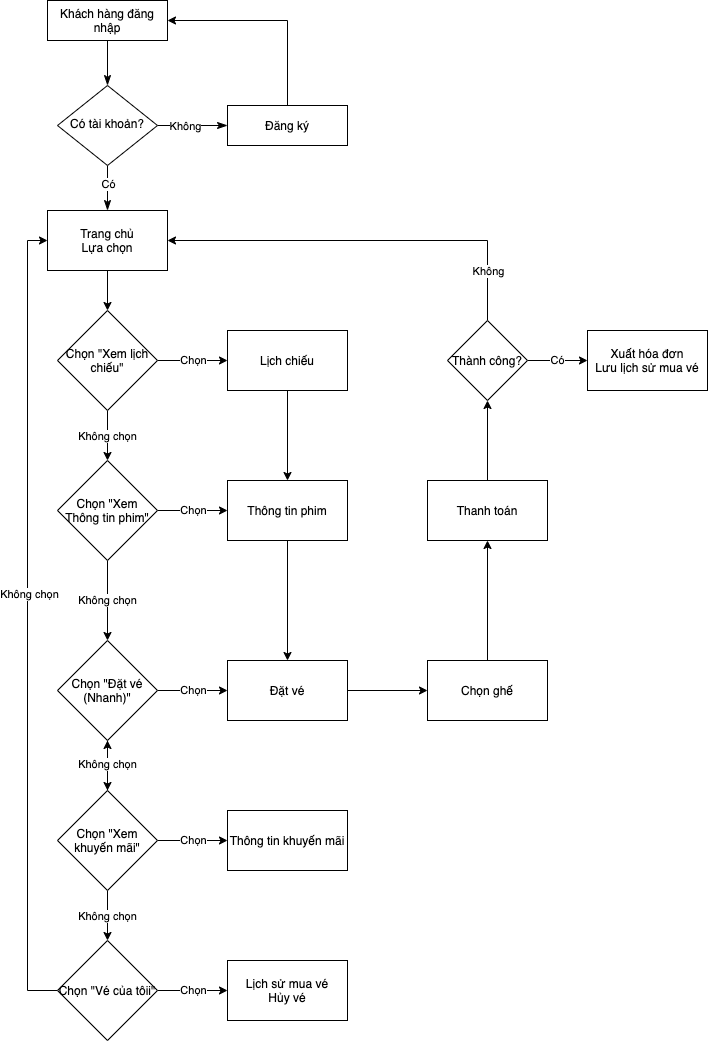
\includegraphics[scale = 0.6]{GCF Charts/GCF_User.png}
		\caption{Luồng điều khiển của Khách hàng}
	\end{center}
\end{figure}

\subsection{Yêu cầu phần cứng}

\begin{itemize}
	\item Phía client: Một máy tính cá nhân, tablet, điện thoại thông minh bất kì có thể sử dụng các trình duyệt web như Google Chrome, Microsoft Edge, Mozilla Firefox, Safari...
	\item Phía server: Máy chủ vật lý hoặc máy chủ ảo có cấu hình tương đương tối thiểu như sau
	\begin{itemize}
		\item CPU: Intel Xeon 2.0 GHz, 2M Cache
		\item RAM: 2GB DDR4
		\item Lưu trữ: 240GB HDD/SSD
		\item Mạng: 100MBps cho cả Upload và Download, không giới hạn băng thông 
	\end{itemize}
\end{itemize}
\clearpage

\section{Biểu đồ lớp}

\subsection{Biểu đồ lớp}

\begin{figure}[H]
	\begin{center}
		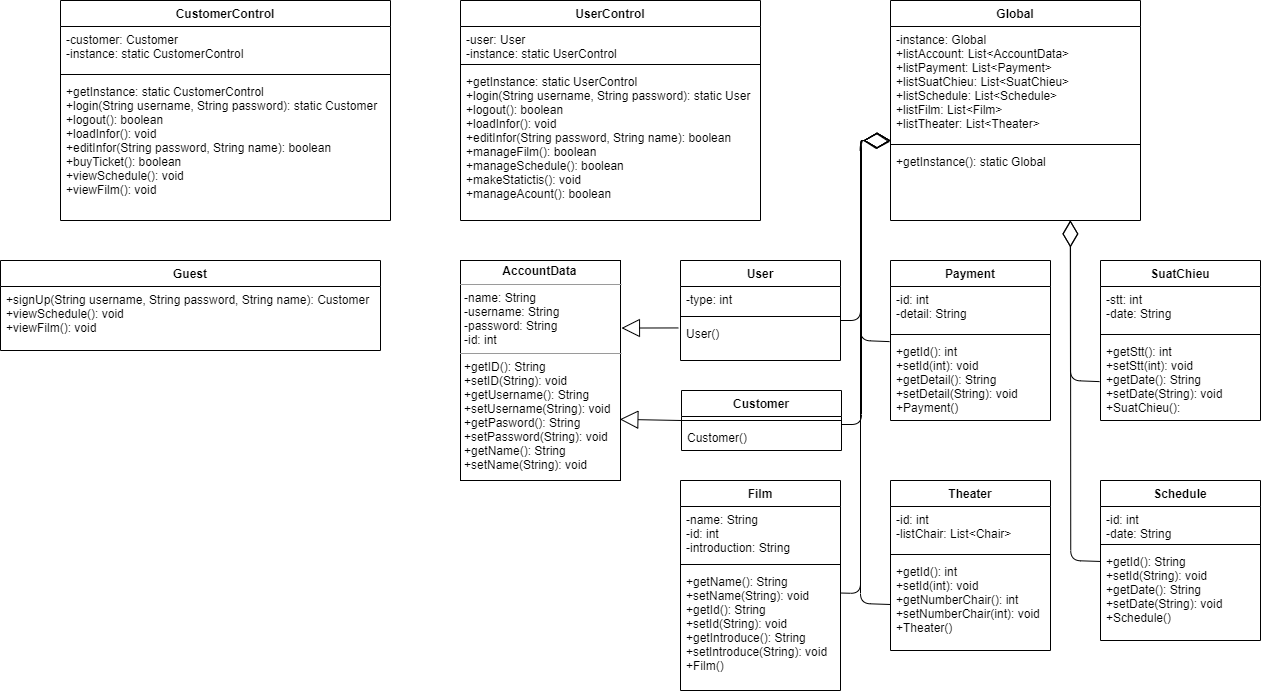
\includegraphics[angle=90,scale=0.49]{image/5.0.png}
		\caption{Class Diagram}
	\end{center}
\end{figure}

\subsection{Đặc tả các lớp}

\subsubsection{Lớp AccountData}
\begin{table}[h]
	\begin{center}
		\begin{tabular}{|c|l|c|l|l|}
			\hline
			STT & \multicolumn{1}{c|}{Tên thuộc tính} & Loại                         & \multicolumn{1}{c|}{Ràng buộc} & \multicolumn{1}{c|}{Ý nghĩa} \\ \hline
			1   & id                                  & \multicolumn{1}{l|}{private} & not null, unique               & Định danh tài khoản          \\ \hline
			2   & name                                & private                      & not null                       & Tên người dùng               \\ \hline
			3   & username                            & private                      & not null, unique               & Xem lịch chiếu               \\ \hline
			4   & password                            & private                      & not null                       & Mật khẩu đăng nhập           \\ \hline
			\end{tabular}
		\caption{Mô tả phương thức lớp AccountData}
	\end{center}
\end{table}

\begin{table}[H]
	\begin{center}
		\begin{tabular}{|c|l|c|l|l|}
			\hline
			STT & \multicolumn{1}{c|}{Tên phương thức} & Loại   & \multicolumn{1}{c|}{Ràng buộc} & \multicolumn{1}{c|}{Ý nghĩa}    \\ \hline
			1   & Các phương thức get, set             & public &             Không                   & Lấy hoặc gán giá trị thuộc tính \\ \hline
			\end{tabular}
		\caption{Mô tả phương thức lớp AccountData}
	\end{center}
\end{table}

\subsubsection{Lớp User - kế thừa lớp AccountData}

\begin{table}[H]
	\begin{center}
		\begin{tabular}{|c|l|c|l|l|}
			\hline
			STT & \multicolumn{1}{c|}{Tên thuộc tính} & Loại    & \multicolumn{1}{c|}{Ràng buộc} & \multicolumn{1}{c|}{Ý nghĩa} \\ \hline
			1   & type                                & private & in\{1:admin,2:quản lí\}        & Loại User(quản lí, admin)    \\ \hline
			\end{tabular}
			\caption{Bảng mô tả thuôc tính lớp User}
	\end{center}
\end{table}

\begin{table}[H]
	\begin{center}
		\begin{tabular}{|c|l|c|l|l|}
			\hline
			STT & \multicolumn{1}{c|}{Tên phương thức} & Loại   & \multicolumn{1}{c|}{Ràng buộc} & \multicolumn{1}{c|}{Ý nghĩa} \\ \hline
			1   & User                                 & public &            Không                    & Khởi tạo đối tượng User      \\ \hline
			\end{tabular}
		\caption{Bảng mô tả phương thức lớp User}
	\end{center}
\end{table}

\subsubsection{Lớp Customer - kế thừa lớp AccountData}

\begin{table}[H]
	\begin{center}
		\begin{tabular}{|c|l|c|l|l|}
			\hline
			STT & \multicolumn{1}{c|}{Tên phương thức} & Loại   & \multicolumn{1}{c|}{Ràng buộc} & \multicolumn{1}{c|}{Ý nghĩa} \\ \hline
			1   & Customer                             & public &         Không                       & Khởi tạo đối tượng Customer  \\ \hline
			\end{tabular}
		\caption{Bảng mô tả phương thức lớp Customer}
	\end{center}
\end{table}

\subsubsection{Lớp Payment}

\begin{table}[H]
	\begin{center}
		\begin{tabular}{|l|l|l|l|l|}
		\hline
		STT & Tên thuộc tính & Loại    & Ràng buộc & Ý nghĩa                  \\ \hline
		1   & id             & private &   not null, unique        & Định danh một thanh toán \\ \hline
		2   & detail         & private &   Không        & Chi tiết một thanh toán  \\ \hline
		\end{tabular}
		\caption{Bảng mô tả thuộc tính lớp Payment}
	\end{center}
\end{table}

\begin{table}[H]
	\begin{center}
		\begin{tabular}{|c|l|c|l|l|}
			\hline
			STT & \multicolumn{1}{c|}{Tên phương thức} & Loại                        & \multicolumn{1}{c|}{Ràng buộc} & \multicolumn{1}{c|}{Ý nghĩa}    \\ \hline
			1   & Các phương thức get, set             & public                      &      Không                          & Lấy hoặc gán giá trị thuộc tính \\ \hline
			2   & Payment                              & \multicolumn{1}{l|}{public} &      Không                          & Khởi tạo một đối tượng Payment  \\ \hline
			\end{tabular}
		\caption{Bảng mô tả phương thức lớp Payment}
	\end{center}
\end{table}

\subsubsection{Lớp SuatChieu}
\begin{table}[H]
	\begin{center}
		\begin{tabular}{|c|l|c|l|l|}
			\hline
			STT & \multicolumn{1}{c|}{Tên thuộc tính} & Loại                         & \multicolumn{1}{c|}{Ràng buộc} & \multicolumn{1}{c|}{Ý nghĩa}        \\ \hline
			1   & stt                                 & private                      & not null                       & Số thứ tự trong ngày của suất chiếu \\ \hline
			2   & date                                & \multicolumn{1}{l|}{private} & not null                       & Ngày khởi tạo suất chiếu            \\ \hline
		\end{tabular}
		\caption{Bảng mô tả thuộc tính lớp SuatChieu}
	\end{center}
\end{table}

\begin{table}[H]
	\begin{center}
		\begin{tabular}{|c|l|c|l|l|}
			\hline
			STT & \multicolumn{1}{c|}{Tên phương thức} & Loại                        & \multicolumn{1}{c|}{Ràng buộc} & \multicolumn{1}{c|}{Ý nghĩa}     \\ \hline
			1   & Các phương thức get, set             & public                      &                 Không               & Lấy hoặc gán giá trị thuộc tính  \\ \hline
			2   & SuatChieu                            & \multicolumn{1}{l|}{public} &                      Không          & Khởi tạo một đối tượng SuatChieu \\ \hline
			\end{tabular}
		\caption{Bảng mô tả phương thức lớp SuatChieu}
	\end{center}
\end{table}

\subsubsection{Lớp Film}

\begin{table}[H]
	\begin{center}
		\begin{tabular}{|c|l|l|l|l|}
			\hline
			STT                     & \multicolumn{1}{c|}{Tên thuộc tính} & \multicolumn{1}{c|}{Loại}    & \multicolumn{1}{c|}{Ràng buộc} & \multicolumn{1}{c|}{Ý nghĩa} \\ \hline
			1                       & name                                & \multicolumn{1}{c|}{private} & not null                       & Tên phim                     \\ \hline
			2                       & id                                  & private                      & not null, unique               & Định danh một bộ phim        \\ \hline
			3			   		    & introduction                        & private                      &         not null                       & Giới thiệu phim              \\ \hline
			\end{tabular}
			\caption{Bảng mô tả thuộc tính lớp Film}
	\end{center}
\end{table}

\begin{table}[H]
	\begin{center}
		\begin{tabular}{|c|l|c|l|l|}
			\hline
			STT & \multicolumn{1}{c|}{Tên phương thức} & Loại                        & \multicolumn{1}{c|}{Ràng buộc} & \multicolumn{1}{c|}{Ý nghĩa}    \\ \hline
			1   & Các phương thức get, set             & public                      &            Không                    & Lấy hoặc gán giá trị thuộc tính \\ \hline
			2   & Film                                 & \multicolumn{1}{l|}{public} &                 Không               & Khởi tạo một đối tượng Film     \\ \hline
			\end{tabular}
			\caption{Bảng mô tả phương thức lớp Film}
	\end{center}
\end{table}

\subsubsection{Lớp Theater}

\begin{table}[H]
	\begin{center}
		\begin{tabular}{|c|l|c|l|l|}
			\hline
			STT & \multicolumn{1}{c|}{Tên thuộc tính} & Loại                         & \multicolumn{1}{c|}{Ràng buộc} & \multicolumn{1}{c|}{Ý nghĩa} \\ \hline
			1   & id                                  & private                      & not null, unique               & Định danh một phòng chiếu    \\ \hline
			2   & listChair                           & \multicolumn{1}{l|}{private} & not null                       & Danh sách ghế                \\ \hline
			\end{tabular}
			\caption{Bảng mô tả thuộc tính lớp Theater}
	\end{center}
\end{table}

\begin{table}[H]
	\begin{center}
		\begin{tabular}{|c|l|c|l|l|}
			\hline
			STT & \multicolumn{1}{c|}{Tên phương thức} & Loại                        & \multicolumn{1}{c|}{Ràng buộc} & \multicolumn{1}{c|}{Ý nghĩa}    \\ \hline
			1   & Các phương thức get, set             & public                      &              Không                  & Lấy hoặc gán giá trị thuộc tính \\ \hline
			2   & Theater                              & \multicolumn{1}{l|}{public} &                   Không             & Khởi tạo một đối tượng Theater  \\ \hline
			\end{tabular}
			\caption{Bảng mô tả thuộc tính lớp Theater}
	\end{center}
\end{table}

\subsubsection{Lớp Schedule}

\begin{table}[H]
	\begin{center}
		\begin{tabular}{|c|l|c|l|l|}
			\hline
			STT & \multicolumn{1}{c|}{Tên thuộc tính} & Loại                         & \multicolumn{1}{c|}{Ràng buộc} & \multicolumn{1}{c|}{Ý nghĩa} \\ \hline
			1   & id                                  & private                      & not null, unique               & Định danh một lịch chiếu     \\ \hline
			2   & date                                & \multicolumn{1}{l|}{private} & not null                       & Ngày khởi tạo lịch chiếu     \\ \hline
		\end{tabular}
		\caption{Bảng mô tả thuộc tính lớp Schedule}
	\end{center}
\end{table}

\begin{table}[H]
	\begin{center}
		\begin{tabular}{|c|l|c|c|l|}
			\hline
			STT & \multicolumn{1}{c|}{Tên phương thức} & Loại                        & \multicolumn{1}{c|}{Ràng buộc} & \multicolumn{1}{c|}{Ý nghĩa}    \\ \hline
			1   & Các phương thức get, set             & public                      &                   Không             & Lấy hoặc gán giá trị thuộc tính \\ \hline
			2   & Schedule                             & \multicolumn{1}{l|}{public} &                       Không         & Khởi tạo một đối tượng Schedule \\ \hline
		\end{tabular}
		\caption{Bảng mô tả phương thức lớp Schedule}
	\end {center}
\end{table}

\subsubsection{Lớp Global}

\begin{table}[H]
	\begin{center}
		\begin{tabular}{|c|l|l|c|l|}
			\hline
			STT & \multicolumn{1}{c|}{Tên thuộc tính} & \multicolumn{1}{c|}{Loại}    & \multicolumn{1}{c|}{Ràng buộc} & \multicolumn{1}{c|}{Ý nghĩa}                                                                             \\ \hline
			1   & instance                            & \multicolumn{1}{c|}{private} & Không                                & \begin{tabular}[c]{@{}l@{}}Đối tượng Global duy nhất được\\ tạo để quản lí dữ liệu toàn cục\end{tabular} \\ \hline
			2   & listAccount                         & public                       & not null                       & Quản lí danh sách các AccountData                                                                        \\ \hline
			3   & listPayment                         & public                       & not null                       & Quản lí danh sách các thanh toán                                                                         \\ \hline
			4   & listSuatChieu                       & public                       & not null                       & Quản lí danh sách các suất chiếu                                                                         \\ \hline
			5   & listSchedule                        & public                       & not null                       & Quản lí danh sách các lịch chiếu                                                                         \\ \hline
			6   & listFilm                            & public                       & not null                       & Quản lí danh sách các phim                                                                               \\ \hline
			7   & listTheater                         & public                       & not null                       & Quản lí danh sách các phòng chiếu                                                                        \\ \hline
		\end{tabular}
		\caption{Bảng mô tả thuộc tính lớp Global}
	\end{center}
\end{table}

\begin{table}[H]
	\begin{center}
		\begin{tabular}{|c|l|c|c|l|}
			\hline
			STT & \multicolumn{1}{c|}{Tên phương thức} & Loại   & \multicolumn{1}{c|}{Ràng buộc} & \multicolumn{1}{c|}{Ý nghĩa}        \\ \hline
			1   & getInstance                          & public & Không                               & Truy xuất đối tượng Global duy nhất \\ \hline
		\end{tabular}
		\caption{Bảng mô tả phương thức lớp Global}
	\end{center}
\end{table}

\subsubsection{Lớp UserControl}

\begin{table}[H]
	\begin{center}
		\begin{tabular}{|c|l|c|c|l|}
			\hline
			STT & \multicolumn{1}{c|}{Tên thuộc tính} & Loại                         & \multicolumn{1}{c|}{Ràng buộc} & \multicolumn{1}{c|}{Ý nghĩa}                        \\ \hline
			1   & user                                & private                      & not null                       & Dữ liệu User của UserControl                        \\ \hline
			2   & instance                            & \multicolumn{1}{l|}{private} &          Không                      & Đối tượng User duy nhất được khởi tạo khi đăng nhập \\ \hline
		\end{tabular}
		\caption{Bảng mô tả thuôc tính lớp UserControl}
	\end{center}
\end{table}

\begin{table}[H]
	\begin{center}
		\begin{tabular}{|c|l|c|c|l|}
			\hline
			STT & \multicolumn{1}{c|}{Tên phương thức} & \multicolumn{1}{c|}{Loại}   & \multicolumn{1}{c|}{Ràng buộc} & \multicolumn{1}{c|}{Ý nghĩa}                       \\ \hline
			1   & getInstance                          & \multicolumn{1}{c|}{public} &       Không                         & Truy xuất đối tượng UserControl duy nhất           \\ \hline
			2   & login                                & public                      &       Không                         & Đăng nhập nếu chính xác trả về một User            \\ \hline
			3   & logout                               & public                      &       Không                         & Đăng xuất, nếu thành công trả về true và ngược lại \\ \hline
			4   & loadInfor                            & public                      &       Không                         & Xem thông tin cá nhân(quản lí)                     \\ \hline
			5   & editInfor                            & public                      &       Không                         & Chỉnh sửa thông tin cá nhân(quản lí)               \\ \hline
			6   & manageFilm                           & public                      &       Không                         & Quản lí phim(Thêm, xóa, sửa)(quản lí)              \\ \hline
			7   & manageSchedule                       & public                      &       Không                         & Quản lí lịch chiếu(Thêm, xóa, sửa)(quản lí)        \\ \hline
			8   & makeStatic                           & public                      &       Không                         & Thống kê doanh thu(Admin)                          \\ \hline
			9   & manageAccount                        & public                      &       Không                         & Quản lí các quản lí(thêm, xóa, sửa)(admin)         \\ \hline
		\end{tabular}
		\caption{Bảng mô tả phương thức lớp UserControl}
	\end{center}
\end{table}

\subsubsection{Lớp CustomerControl}

\begin{table}[H]
	\begin{center}
		\begin{tabular}{|c|l|l|c|l|}
		\hline
		STT & Tên thuộc tính & Loại    & Ràng buộc & \multicolumn{1}{c|}{Ý nghĩa}                                           \\ \hline
		1   & user           & private &    not null       & Dữ liệu user của UserControl                      \\ \hline
		2   & instance       & private &         Không  & Đối tượng user duy nhất được tạo ra khi đăng nhập \\ \hline
		\end{tabular}
		\caption{Bảng mô tả thuộc tính lớp CustomerControl}
	\end{center}
\end{table}

\begin{table}[H]
	\begin{center}
		\begin{tabular}{|c|c|l|c|l|}
		\hline
		STT & Tên phương thức & Loại   & Ràng buộc & \multicolumn{1}{c|}{Ý nghĩa}                                      \\ \hline
		1   & getInstance     & public &   Không        & Truy xuất đối tượng CustomerControl          \\ \hline
		2   & login           & public &   Không        & Đăng nhập, nếu chính xác trả về một Customer \\ \hline
		3   & logout          & public &   Không        & Đăng xuất, nếu đúng trả về true và ngược lại \\ \hline
		4   & loadInfor       & public &   Không        & Xem thông tin cá nhân                        \\ \hline
		5   & editInfor       & public &   Không        & Chỉnh sửa thông tin cá nhân                  \\ \hline
		6   & buyTicket       & public &   Không        & Mua vé                                       \\ \hline
		\end{tabular}
		\caption{Bảng mô tả phương thức lớp CustomerControl}
	\end{center}
\end{table}

\subsubsection{Lớp Guest}

\begin{table}[H]
	\begin{center}
		\begin{tabular}{|c|l|l|c|l|}
		\hline
		STT & Tên phương thức & Loại   & Ràng buộc & \multicolumn{1}{c|}{Ý nghĩa}                                 \\ \hline
		1   & login           & public &   Không        & Đăng nhập, nếu đúng trả về một Customer \\ \hline
		2   & viewSchedule    & public &   Không        & Xem lịch chiếu                          \\ \hline
		3   & viewFilm        & public &   Không        & Xem phim                                \\ \hline
		\end{tabular}
		\caption{Bảng mô tả thuộc tính lớp Guest}
	\end{center}
\end{table}

\clearpage

\section{Quản trị dự án và kế hoạch làm việc}

\subsection{Tổng hợp đóng góp từ các thành viên của nhóm}

Các vấn đề mà nhóm đang đối mặt và hướng giải quyết tương ứng
\begin{enumerate}
    \item Thành viên nhóm không cập nhật thường xuyên yêu cầu
    \begin{itemize}
        \item Mô tả vấn đề: Khi có task mới hoặc lưu ý mới được cập nhật trên Trello, các thành viên không thường xuyên kiểm tra Trello việc cập nhật thông tin bị muộn
        \item Hướng giải quyết: Khi có lưu ý hoặc có task mới, người đưa ra task phải chủ động gửi tin nhắn cho nhóm để thông báo về cập nhật
    \end{itemize}

    \item Không xác định rõ sự phụ thuộc giữa các task
    \begin{itemize}
        \item Mô tả vấn đề: Khi nhận task, các thành viên trong nhóm chọn task của mình, ước lượng thời gian làm việc và đặt deadline cho từng chức năng mà không quan tâm đến việc task này phụ thuộc vào một hoặc nhiều task khác. Điều này dẫn đến việc tận dụng không hiểu quả thời gian làm việc
        \item Hướng giải quyết: Sau khi mỗi cá nhân tự nhận task, nhóm tiến hành meeting để xác định sự phụ thuộc giữa các task. Từ đó đưa ra deadline cụ thể và chính xác hơn
    \end{itemize}

    \item Không thống nhất được kết quả làm việc của các task 
    \begin{itemize}
        \item Mô tả vấn đề: Trong quá trình làm việc song song, các thành viên thực hiện các task riêng lẻ nhưng giữa các task có sự phụ thuộc lẫn nhau. Tuy nhiên, giao tiếp giữa các thành viên trong team lại rất hạn chế nên thường xảy ra việc không đồng nhất trong kết quả làm việc
        \item Hướng giải quyết: Sau khi xác định được sự phụ thuộc giữa các task, các thành viên đảm nhiệm task đó phải làm việc riêng với nhau và thống nhất kết quả chung
    \end{itemize}

    \item Một thành viên nhận 1 task quá lớn, bao gồm nhiều task con
    \begin{itemize}
        \item Mô tả vấn đề: Khi một thành viên trong nhóm nhận 1 task quá sức với bản thân. Hơn nữa, task này còn được nhiều task khác phụ thuộc vào. Khi thành viên này không hoàn thành đúng tiến độ sẽ làm ảnh hướng đến rất nhiều task khác
        \item Hướng giải quyết: Chia task lớn thành các task nguyên tố (không thể chia nhỏ hơn)
    \end{itemize}
\end{enumerate}

\subsection{Báo cáo tiến độ và điều phối dự án}

Hiện tại dự án đang đi đúng tiến độ trong kế hoạch được đặt ra tại báo cáo \#1

\subsection{Kế hoạch thực hiện}

\begin{figure}[H]
	\begin{center}
		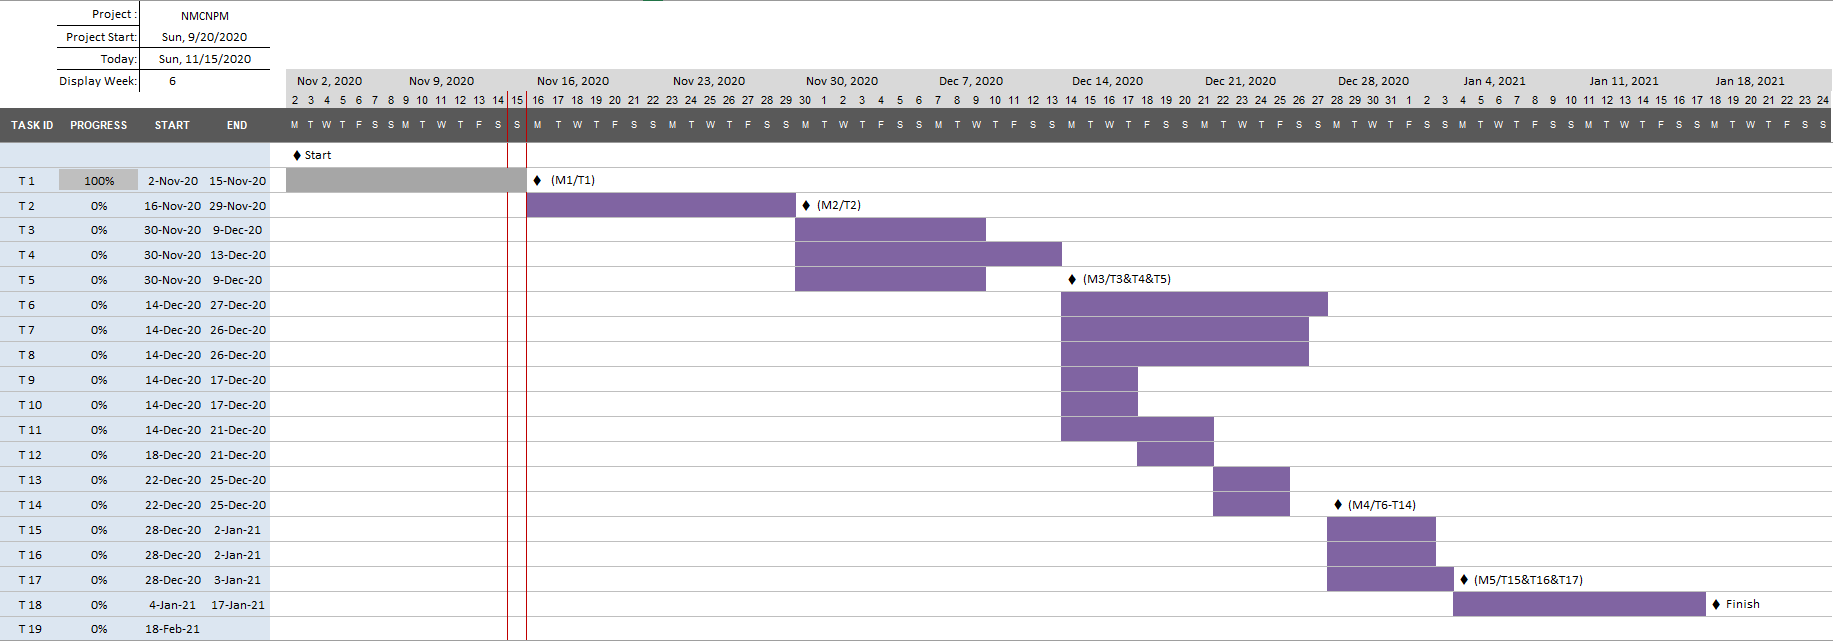
\includegraphics[scale=0.35, angle=90]{image/gantt.png}
		\caption{Activity bar chart}
	\end{center}
\end{figure}

\subsection{Phân rã trách nhiệm (Breakdown of Responsibilities)}

\begin{itemize}
	\item Phân chia vai trò chính trong mỗi module
	\begin{itemize}
		\item 
	\end{itemize}

	\item Điều phối tích hợp
	\begin{itemize}
		\item Trong quá trình tích hợp, các thành viên đều phải tham gia
		\item Người chịu trách nhiệm chính trong quá điều phối trình tích hợp là: Phạm Tống Bình Minh - Vai trò: Developer
	\end{itemize}

	\item Kiểm thử tích hợp
	\begin{itemize}
		\item Việc cài đặt unit test cho các phần phải được thực hiện bởi thành viên chịu trách nhiệm cài đặt phần đó
		\item Người chịu trách nhiệm chính trong quá trình kiểm thử tích hợp là Nguyễn Duy Vũ - Vai trò: Tester
	\end{itemize}
\end{itemize}

\clearpage

\section{Tham khảo}
\clearpage
	
\end{document}